\documentclass[11pt]{article}
\usepackage[paperwidth=12cm, paperheight=18cm, margin=1cm]{geometry}
\usepackage{amsmath, tikz}
\pagestyle{empty}

\begin{document}
\begin{center}
  {\LARGE\bfseries Simpson's Paradox}\\[4pt]
  {\large Better in every group, worse overall}
\end{center}

A real study of kidney stone treatments (1986) compared
open surgery (A) with a less invasive procedure (B).

\section*{Success rates}
\begin{center}
\begin{tabular}{lcc}
  \hline
  Stone size & Treatment A & Treatment B \\
  \hline
  Small & \textbf{93\%} (81/87) & 87\% (234/270) \\
  Large & \textbf{73\%} (192/263) & 69\% (55/80) \\
  \hline
  All & 78\% (273/350) & \textbf{83\%} (289/350) \\
  \hline
\end{tabular}
\end{center}

A wins for small stones \emph{and} for large stones, yet B
wins overall. How?

\begin{center}
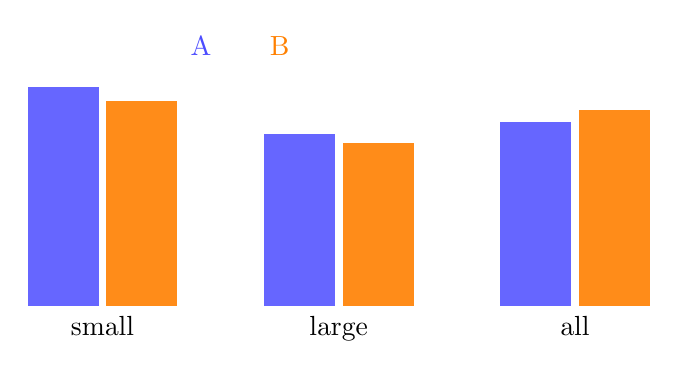
\begin{tikzpicture}[yscale=3]
  \foreach \x/\a/\b/\name in {0/0.93/0.87/small, 3/0.73/0.69/large, 6/0.78/0.83/all} {
    \fill[blue!60] (\x,0) rectangle +(0.9,\a);
    \fill[orange!90] (\x+1,0) rectangle +(0.9,\b);
    \node[below] at (\x+0.95,0) {\name};
  }
  \node[blue!70] at (2.2,1.1) {A};
  \node[orange] at (3.2,1.1) {B};
\end{tikzpicture}
\end{center}

\section*{The hidden variable}
Doctors gave A the hard cases: most large stones got A.
\[
  \frac{81 + 192}{87 + 263} < \frac{234 + 55}{270 + 80}
\]
\centerline{\bfseries Aggregating data can reverse the truth.}
\end{document}
